
% Background and Significance
% No page limit
\chapter{Introduction}
\label{chap_intro}
\begin{quote}
{\em ``The brain is the last and grandest biological frontier, the most complex thing we have yet discovered in our universe. It contains hundreds of billions of cells interlinked through trillions of connections. The brain boggles the mind.''}  

--James D. Watson, Discovering the Brain, National Academy Press, 1992
\end{quote}

The human brain serves as the control center of the nervous system and controls nearly every activity that is required for survival. It contains hundreds of billions of neurons that communicate with each other via a network of hundreds of trillions of connections, forming the most complex organ in the human body. Having been recognized as the body's major controlling center by the Greek physician Hippocrates, the brain has long been a focus of scientific inquiry~\cite{Finger2005}. Early examinations centered upon dissection to examine the neuroanatomy of the brain and led to the discovery of critical features of the brain, such as Andreas Vesalius' distinction between gray and white matter~\cite{Vesalius1543} and Joseph Gall's proposal that the brain is composed of many ``organs" each responsible for specific functional faculties~\cite{Gall1810}. Paul Broca's (1824 - 1880) cortical lesion analyses provided critical knowledge as they introduced the concept of functional lateralization and suggested a direct link between structure and function in the brain.  While these ex-vivo examinations of the brain provided great insight into brain anatomy and structure, the ability to examine brain function in-vivo confirmed the functional specialization of subregions of the brain. The study of function also revealed that the functional subregions of the brain to together to form large-scale neural networks that allow for complex cognitive processes. Hence, it is important to not only characterize the anatomy, structure and function in the brain, but also the inter-relations, or connectivity and their influence upon cognitive performance.

In this dissertation, we present methods to quantitatively characterize the relationships between anatomy, structure, and function throughout the human brain through the use of neuroimaging techniques. We use the functional outcome of brain injury to guide an examintion of structural damage in the brain.  We examine both structural and functional connectivity to examine their role in modulating behavior in healthy human brain, and we explore the influence of aging upon lateralization of the brain for both structure and function. In this chapter, we provide background information for the various concepts discussed later, and introduce the reader to the layout and direction of the dissertation.

\section{Normal brain anatomy and physiology}
Due to the compartmentalized nature of the brain, its anatomy may described in a hierarchical manner. The two hemispheres of the human brain have three primary components (1) the hindbrain provides communication between the brain and the rest of the nervous system and is primarily responsible for coordinating involuntary movement; (2) the midbrain connects the hindbrain to the forebrain, and contains several pathways important to hearing and vision; (3) the forebrain is the largest component and is made of up the cerebrum whose functions include thinking, reasoning and remembering as well as the diencephalon which controls all the autonomic regulatory activities of the body such as temperature, hunger, and emotion. The gray matter of the cerebral cortex is the primary component of the cerebrum while the underlying cerebral white matter provides the network of connections between gray matter regions. Each cerebral hemisphere consists of four lobes (figure \ref{fig:brainanatomy}b). The frontal lobe functions involve the ability to recognize future consequences resulting from current actions, suppress unacceptable social responses, and determine similarities and differences between entities or events. The parietal lobe plays important roles in integrating sensory information from various parts of the body, knowledge of numbers and their relations, in the manipulation of objects, and portions of the parietal lobe are involved with visuospatial processing. The temporal lobe is involved in auditory processing, is also important for the processing of semantics in both speech and vision, and plays a key role in the formation of long-term memory. The occipital lobe is the visual processing center of the brain. Further subdivision of the lobes based upon cytoarchitectural features of gray matter, most notably by Brodmann~\cite{Brodmann1909}, has provided a common anatomical frame of reference for studies of anatomy and have been found to correspond to functional specialization.

\begin{figure}
\begin{center}
$\begin{array}{ccc}
\centering
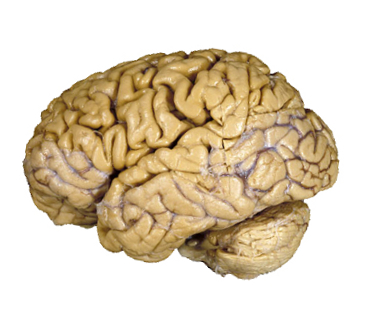
\includegraphics[width=0.3\linewidth]{figures/exvivobrain.jpg} &
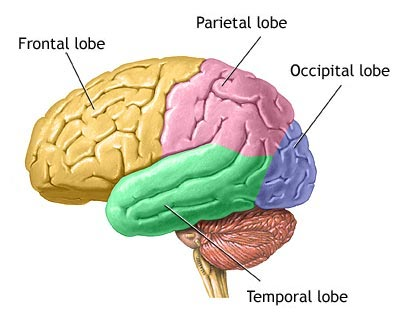
\includegraphics[width=0.3\linewidth]{figures/brainlobes.jpg} &
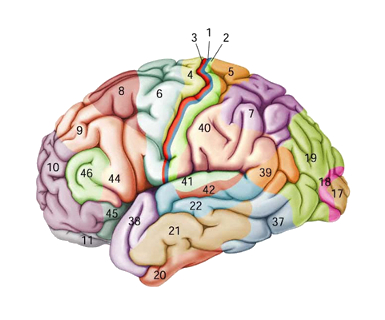
\includegraphics[width=0.3\linewidth]{figures/brodmann.jpg} \\
a) & b) & c)
\end{array}$
\caption{a) An image of an ex-vivo human brain in which the forebrain and hindbrain are visible (image adapted from~\cite{exvivobrain}) b) Each hemisphere of the the forebrain is divided into four lobes as illustrated here (image adapted from~\cite{medlineplus}) c) Brodmann proposed a labeling of the brain surface based upon cytoarchitectural features of the brain (image adapted from~\cite{mcgillbrain})}.
\label{fig:brainanatomy}
\end{center}
\end{figure}

The anatomy of the cerebral white matter is important as it provides the communication network that allows the functional subregions of the cortex to communicate with each other and consists of three types of fibers: (1) projection fibers connect the cortex with the lower parts of the brain and the spinal cord (figure \ref{fig:sketches}a). (2) commisural fibers connect the two hemispheres of the brain (figure \ref{fig:sketches}b). (3) association fibers unite different parts of the same cerebral hemisphere. There are two types of association fibers: (1) those connecting adjacent gyri, short association fibers (i.e.\ u-fibers); (2) those passing between more distant parts, long association fibers. The ability to identify functionally specific subregions of the cortex and the white matter pathways that connect them provides a full anatomical description of specialized neural networks such as the language, memory and visuospatial networks. 

\begin{figure}
\begin{center}
$\begin{array}{ccc}
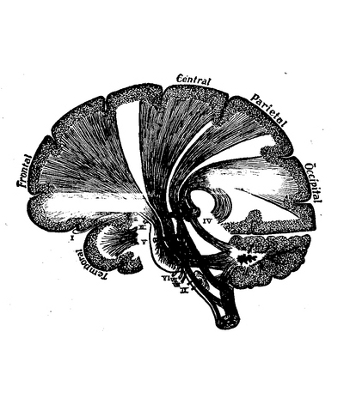
\includegraphics[width=0.3\linewidth]{figures/projectionfiberssketch2.jpg} &
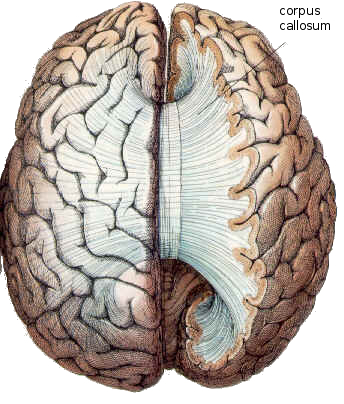
\includegraphics[width=0.3\linewidth]{figures/corpuscallosumsketch.jpg} &
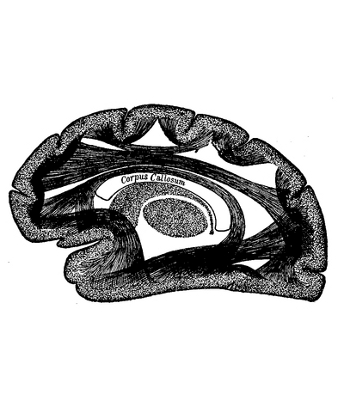
\includegraphics[width=0.3\linewidth]{figures/associationfibersketch2.jpg} \\
a) & b) & c)
\end{array}$
\caption{
Cortical regions communicate via the white matter which consists of: a) the projection fibers that connect the cortex to the lower brain and spinal cord (image adapted from~\cite{gutenberg}) b) The commisural fibers that connect the hemispheres of the brain (image adapted from~\cite{carleton}) c) the association fibers the provide both long and short range intra-hemispheric connections (image adapted from~\cite{gutenberg}).}
\label{fig:sketches}
\end{center}
\end{figure}

\section{Connectivity in the brain}
The human brain is a system comprised of more than $10^{10}$ neurons that provide great computational capacity via a complicated communication network consisting of both local circuits and long-range fiber pathways~\cite{Hagmann2008}. The neurons of the cortical gray matter are responsible for processing information while their axons comprise the white matter that provides the communication channels between the functionally and structurally segregated subregions of the cortex. The study of brain connectivity seeks to understand the anatomical arrangement, structural properties, interconnections, and functional relationships of the elements of this system and is essential for further insight into the nature of cognitive processes and could provide a critical window onto development, aging and neurodegenerative disease in the brain.

\subsection{Anatomical and Structural Connectivity}
The terms anatomical connectivity and structural connectivity are sometimes used interchangeably, but here we distinguish between the two in an attempt to explore the relationship between them as well as the extent to which each relates to functional connectivity. Anatomical connectivity identifies the presence of a physical connection between distinct regions in the brain and quantifies the geometry of the regions and the pathways that connects them. Structural connectivity is concerned with the biophysical properties of the tissue that connects the regions. Collectively, anatomical and structural connectivity are known as the human connectome and they comprehensively describe the biological network of elements that define the human brain~\cite{Hagmann2008}. 

% Anatomic connectivity
Brain development plays an important role in defining the geometry and topography of anatomical connections.
Phylogenetically older brain regions develop first and have direct, sometimes unidirectional, connections~\cite{Gogtay2004b}. The connections typically have a linear configuration as seen in the corticospinal tracts and the thalamo-cortical network. Cortical regions associated with more complex neural networks that require a higher degree of interconnectivity develop later and consist of systems in which subregions may be connected directly or indirectly via intermediary cortical regions. While functional regions of the cortex have been well defined from lesion and functional studies, white matter connective pathways are not as clearly defined due to these indirect and parallel connections. This can lead to confusion and ambiguity regarding the components that comprise a particular neural network. A greater understanding of the inter-relations between anatomy and function in the brain could help identify the components that are relevant to a functionally specific network.

%Structural Connectivity
Structural connectivity examines the architectural properties of anatomical connections in order to estimate the integrity or efficacy of the connections. As with anatomic connectivity, brain development plays an integral role in defining structural connectivity. In addition to temporal variance of maturation, white matter also exhibits spatial variation with maturation first occuring centrally and then peripherally, and from the occipital lobe to the frontal lobe~\cite{Gao2009}. The myelin sheath that surrounds the axons of the white matter provides insulation that enhances the speed at which signals are transmitted by the fibers. Degree of myelination provides the basis for many meaures of structural integrity and the spatial arrangement of myelin sheaths provides a basis for elucidating fiber orientation.

Gall and Spurzheim~\cite{Gall1810} were the first to establish that white matter consists of individual fibers that are grouped into tracts that provide a biological connection between cortical gray matter regions. The myelin sheath that surrounds axons was first described by Thomas Schwann~\cite{McHenry1969}, but the term `myelin' itself was introduced later by neuropathologist Rudolph Vircho~\cite{Morell1980}. Carl Weigert's development of a histological stain for the identification of myelin was critical to advancing the study of white matter and is still is use today~\cite{McHenry1969}. Further work in histological staining techniques by Camillo Golgi provided the ability to visualize entire nerve cells, including the dendritic tree~\cite{Golgi1885}. This technique was employed extensively by Santiago Ram{\'{o}}n y Cajal to study nerve cells in the brain and spinal cord~\cite{Glickstein2006}. The work of Paul Flechsig (1847-1929) greatly advanced knowledge regarding white matter as he was the first to observe that myelination during development varied based upon anatomical location and he also introduced Flechsig' rule, stating that cortical sensory areas are not directly connected with each other, but rather connect to adjacent association cortices~\cite{Flechsig1901}, a concept that profoundly influenced modern neuroscientific concepts related to cortical localization. The development of horseradish peroxidase (HRP) tract-tracing allowed for the precise identification of neural pathways in ex-vivo~\cite{Mesulam1982}. More recently, magnetic resonance imaging (MRI) has allowed for routine imaging of gray and white matter and these methods are discussed in more detail in chapter 2. 

\subsection{Functional Connectivity}
The functional organization of the brain seems to obseve two guiding principles: functional segregation and functional integration~\cite{Tononi1994}. Functional segregation refers to the organization and grouping of functionally specialized neurons into spatially distinct cortical brain regions. However, in order to perform complex tasks it is necessary for several functionally segregated and anatomically distinct regions to work together and form functional networks under a concept known as functional integration. Further understanding of brain function requires not only knowledge about the functional topography of the brain but also the complex processes by which these regions interact. Functional segregation and integration and both central to the study of functional connectivity. Functional connectivity has been refered to as an `elusive concept' due to the large variety of defintions, modalities and methods that have been described using this term~\cite{Horwitz2003}. Here we will reserve the term `functional connectivity' to refer to statistical paradigms that identify temporally coordinated activity in spatially distinct units within an individual's brain~\cite{Rykhlevskaia2008}.

Early work examining Gall's theory of functional segregation focused upon cortical lesion studies. In particular, the work of Paul Broca (1824 - 1880) provided evidence for the localization and lateralization of language procesing through post-mortem autopsy of patients who had been unable to pronounce individual words but were unable to produce grammatically correct sentences, a condition later named ``Broca's aphasia." Further work in the language system by Karl Wernicke (1848 - 1905) recognized that not all language deficits resulted from lesions in the cortical region identified by Broca. Through lesion analysis Wernicke identified a cortical region that when damaged prevented subjects from speaking, but did not impede their ability to understand language. The proposal that multiple functionally specific cortical regions work together to perform complex tasks is the basis of functional integration. Additionally, this proposal predicted the importance of structural connectivity as it recognized the critical role of the biological connections between functional regions. Norman Geschwind (1926 - 1984) expanded upon Wernicke's model of the language network and theorized the existence of a parallel pathway connecting Broca's and Wernicke's areas that incorporates an additional cortical region. More recently, additional evidence for functional segregation has been provided by a variety of techniques including PET~\cite{Zeki1991}, electrophysiology~\cite{Gevins1999} and functional MRI (fMRI)~\cite{Howard1996}. Neuroimaging continues to be used extensively to study functional integration and functional connectivity~\cite{Sporns2007B} and these methods are discussed in more detail in chapter 2.

%\subsection{Effective Connectivity}
%Effective connectivity is defined as `the influence that one neural system exerts over another either directly or indirectly'~\cite{Friston1993}. Studies of effective connectivity utilize methods that employ statistical models and make anatomical assumptions to restrict the analysis to a subset of functional regions. The incorporation of anatomical assumptions provides an opportunity for a combined analysis of functional, anatomical and structural connectivity. Unlike functional connectivity measures that attempt to measure what the brain is doing, effective connectivity examines how the brain is working. Studies of effective connectivity rely upon neuroimaging methods and chapter 2 reviews the approaches that have been proposed for modeling the dynamics of cortical circuits.

%First developed for use in econometrics, structural equation modeling (SEM) has been applied to the study of effective connectivity~\cite{McIntosh1994}. These models incorporate directed connections between cortical regions to ascribe causal relationships. Two major limitations of SEMs are the (1) reliance upon correlations matrices that limits the number of connections and (2) inability to incorporate temporal information. To address these deficiencies, dynamic causal models (DCM) were proposed by Friston, et al.\ \cite{Friston2003}. The causal model utilised in DCMs allow for interregional and self connections that results in changes in blood flow, volume, and deoxyhemoglobin (dHb) content. These parameters, all of which contribute to the BOLD fMRI signal, are quantified by DCM.  DCM is currently limited by the computationally demanding model fitting that limits the analysis to small number of regions.


\section{Introduction to the dissertation}

Here we present novel approaches for examining connectivity in the brain. We focus on connectivity at the macro scale and how it may be studied with MRI. To this end, we use diffusion tensor MRI along with fiber tractography to extract anatomical and structural information from white matter fiber bundles. We demonstrate the ability of these methods to identify both local and gross white matter properties. Atlas-based techniques are used to define geometric models of white matter fiber pathways. These models are used to identify the white matter fiber tracts that provide the anatomical connectivity that provides communication between the nodes of a functional network defined using fMRI. Meaures of structural and functional connectivity are related to cognitive performance in a language-based decision making task. 

Chapter~\ref{chap_back} presents background on methods for using neuroimaging to study connectivity in the human brain.  Chapter~\ref{chap_tbi} focuses on using fiber tractography to examine an a priori functionally-based hypothesis regarding localized structural differences in a population of subjects whom have suffered a traumatic brain injury (TBI). Chapter~\ref{chap_homo} describes an examination of both structural and functional connectivity in a healthy young adult population and relates these measures to cognitive performance. In chapter~\ref{chap_lat} we discuss a study of lateralization in the brain and examine the influence of aging on both structure and function. Finally, in chapter~\ref{chap_conclusions}, we discuss the findings described in this dissertation and interesting questions to be investigated in the future.

%Chapter 3 dicusses the use of fiber tractography for examining the topography of inter-hemispheric cortical connectivity and evaluates schemes for anatomical connectivity based partitioning of the mid-sagittal cross-section of the corpus callosum.

%The anatomical frame-of-reference provided by the fiber model is used to develop metrics that incorporate the  eometry of the model and quantify how it related to the underlying structure in individual subjects. 
%We demonstrate the ability of these methods to identify both local and gross white matter differences and characterize difference types of connective pathologies and the metrics appropriate for their investigation. Finally, a healthy control atlas is used to model the language network in order to explore the relationship between functional and structural connectivity in a well-known sub-network of the brain and demonstrate how they may be used to identify the most likely candidate when multiple network configurations are possible. Performance in a task-based functional experiment is used to characterize the contributions of the different types of connectivity to cognitive performance.



%
%
%
% From proposal
%
%
%


%Paragraph discussing brain as a computational network


% DTI and structural connectivity
%\section{Diffusion Tensor MRI}
%Of particular interest in this work is the use of diffusion tensor MRI in the examination of structural connectivity. Diffusion tensor imaging provides an \emph{in-vivo} non-invasive measure of the local probability of self-motion of water molecules and has proven useful in a number of applications for the study of brain white matter~\cite{Basser1994}. 
%The diffusion of water in white matter is highly anisotropic due to cell walls and myelin which inhibit diffusion perpendicular to the fiber tracts more so than diffusion parallel to the tracts. Both the shape and orientation of the diffusion tensor provide important information regarding the structure of the white matter. Scalar metrics derived from the diffusion tensor, such as fractional anisotropy (FA) and mean diffusion (MD) are often used to quantify various tissue properties. The structural information provided by the diffusion tensor has been shown to be useful in a multitude of studies examining topics such as neurodegenerative disorders, traumatic brain injury, development, and ageing among others~\cite{Lebel2008,Sydykova2007,Xu2007}.


%\section{Structural Connectivity}
%Recently, a number of studies have sought to use DTI to measure whole brain structural connectivity~\cite{Honey2009,Hagmann2008,Hagmann2007,Sporns2005,Iturria-Medina2007}. Many of these studies have relied upon measures such as "fiber counts" and fiber length to estimate structural connectivity. These types of metrics are known to be unreliable due to bias resulting from total brain volume, differences in size between regions of the brain, noise, and partial voluming~\cite{Corouge2006}. Additionally, they fail to incorporate the geometric features provided by the tract model as well as neglecting to incorporate the biophysical properties of the tissue that compromises these fiber pathways. The use of metrics for structural connectivity that leverage the anatomic framework provided by tractography to probe underlying tissue architecture may provide more relevant insight regarding the physical integrity of cortical connections. 

%The examination of cortical thickness provides an alternative method for examining structural connectivity between cortical regions~\cite{Lerch2006,He2007,He2008}. This approach is similar to methods for examining functional connectivity where a seed region-of-interest is used to test for statistical dependence with other point in the cortex. Here however, measures of cortical thickness are compared. An examination of the language network revealed a connectivity pattern that closely resembles the results of fiber tractography studies~\cite{Lerch2006} and a study of Alzeheimer's disease provided evidence of large-scale disruption of integrity in brain networks~\cite{He2008}.

%%Paragraph discussing graph based analysis of the brain network
%\section{Graph-based Analysis of Connectivity}
%The use of graph-based network analysis techniques provides a natural, and increasingly popular, framework for examining connectivity in the brain~\cite{Hagmann2007,Iturria-Medina2007,Iturria-Medina2008,Hagmann2008,Honey2007,Achard2006}. The vertices of the graph correspond to functionally related sets of neurons while the edges correspond to the physical connection or statistical dependencies between these nodes. Much previous work used this concept to study functional connectivity but recently a great deal of work has focused upon incorporating both structural and functional connectivity into a common network for analysis~\cite{Werring1998a,Werring1999b,Wieshmann2001,Honey2009,Bullmore2009,Koch2002a,Skudlarski2008}. Vertices may interact via multiple connections with variable length or weights assigned to them as well as through indirect paths that pass through other vertices. This representation provides a multitude of methods for examining the data such as clustering, path lengths, vertex degree and strength and many others~\cite{Brandes2005}. This framework additionally provide a natural basis for examination at multiple scales. 

%% How we address the above work with novel work
%\section{Significance of Proposed Work}
%Here we present  a framework for examining connectivity in the brain. We focus on connectivity at the macro scale and how it may be studied with MRI. To this end, we using diffusion tensor MRI along with fiber tractography to extract structural information from white matter fiber bundles. The anatomical frame-of-reference provided by the fiber model is used to develop metrics that incorporate the geometry of the model and quantify how it related to the underlying structure in individual subjects. 
%We demonstrate the ability of these methods to identify both local and gross white matter differences and characterize difference types of connectivity pathologies and the metrics appropriate for their investigation. Finally, a healthy control atlas is used to model the language network in order to explore the relationship between functional and structural connectivity in a well-known sub-network of the brain.













